\section{Estimating the Transmit Power of Transmitters}
\label{sec:power}

In this section, we extend our techniques to estimate the transmit power of the
intruders; we refer to the overall problem as  Multiple Transmitter Power Estimation (\mtpe). Estimation of the transmit power of transmitters can be very useful in the shared
spectrum systems. In particular, estimated transmit powers of the primary users (if unknown, as in the case of military users or legacy systems) can be used to set a
``protective" region around them---inside which secondary users can be disallowed~\cite{Ureten2011powerlocation}.
%%%%%%%
Estimating transmit power of secondary users can also be useful. E.g., if the violation
in a shared spectrum system is based on a certain minimum threshold, then it is important to estimate the transmit power to determine a violation. 
Also, the estimated transmit power of secondary users can also be used to ``circumvent" their intrusion---i.e., for the primary users to appropriately increase their transmit power to overcome the harmful interference from the secondary users. 
%%%%%%%%
In general, estimating the transmission power is beneficial to various operations such as node localization, event classification, jammer detection \cite{PowerEstimate2010Zafer}.
 
There are several works that estimates the transmission power of a single transmitter, often jointly with its location \cite{PowerEstimate2010Zafer, Ureten2011powerlocation, icoin2007-powerposition}.
Our previous work \cite{ipsn20-mtl} can estimate the power of multiple transmitters.
The similarity among all four of these methods is that they are estimating the power and location jointly.
In this paper, we propose a new method that leverages the capabilities of \our by using it as a building block. We first localize the transmitters by \our. 
Then given the localized locations, estimate the transmitters' transmission power by a newly designed CNN model \power. 
Although \power is designed to only estimate the power of a single transmitter, we use it together with a machine learning-based error correction method that can mitigate the errors while applying \power to the multiple transmitter power estimation scenario.

In this section, we develop a technique to predict the transmission powers of the intruders. Here, for simplicity, we assume no background authorized users, though, the techniques in this section also work in the presence of authorized users. 
%%%%%%
We leverage our accurate and robust localization solver that tolerates varying transmission power for different transmitters (the varying transmission power needs to be in a range).
We propose an efficient approach and its overall methodology at a high-level is as follows.
And then in the next subsection we describe our \power model.
%%%%%%%%
\begin{enumerate}
\item We use \our to localize the multiple transmitters in a field. 
\item We develop a CNN model \power to predict power of a single isolated (far away from other intruders) intruder. 
\item For other (non-isolated) intruders, we still use \power to predict their powers but employ a post-processing ``correction" technique to account for nearby intruders. 
\end{enumerate}
%%%%%%%%%%%%%%%%%%%


\subsection{\power: Predicting Power of a Single Isolated TX}
\label{subsec:in-out-design}

\softpara{\power Input Image}. 
Let us consider an ``isolated" transmitter $T$. 
To predict $T$'s power, we start with
creating a smaller-size image by cropping the original sensor readings image with the area of a certain size around $T$. 
%%%%%%
In our evaluations in Section \ref{sec:evaluation}, the transmitters have a transmit radius\footnote{I.e., sensors beyond a distance of 20 pixels away from a transmitter $x$ receive only negligible power from $x$.}
of around 20 pixels, which is equivalent to 200 meters.\footnote{Transmission ranges of a standard 2.4 GHz and 5 GHz WiFi at default transmission powers (100 mW) are roughly 45m and 15m respectively. 
In our simulations (Section \ref{sec:evaluation}), we use the 600 MHz frequency band. 
As the lower the signal frequency, the higher the transmission range, a transmission range of around 200m is reasonable.}
For this setting, we used an cropped area of $21 \times 21$ around the isolated transmitter $T$ to predict its power, with $T$ is at the center of this area; also, in this setting, we define a transmitter to be {\em isolated} if there is no other transmitter within a 20-pixel 
distance.\footnote{Ideally, transmitters with a transmit radius of 20 pixels should entail defining isolated transmitters as ones that have no other transmitters within a 40-pixel distance, and then use a
$41\times41$ area around the isolated transmitter. However, in our evaluations, our chosen values yielded a more efficient technique with sufficient accuracy.}
%%%%%%%% 
%%%%%%%%%%%%%%%%%
% We choose a $21 \times 21$ cropped size \blue{because this size is large enough to cover {\em most} surrounding sensors that receive power from the transmitter. 
% %%%%%%%%%%%%
% A larger cropped size, such as $41 \times 41$ grid, will contain {\em all} surrounding sensors that receive power from the transmitter, but will also likely contain some sensors at the edge of this cropped grid who will receive more power from the other transmitters in the case where the transmitters are not ideally isolated (which will happen in reality).}
% So cropping the input to a smaller size will decrease the complexity of the neural network model, thus making the model easier to train.
Note that the above cropping process requires the location of the transmitter to be known, and hence, we undertake the above power-estimation process after the localization of the transmitters using the \our model.  
%%%%%%%%%%%%%%%%%%%%%%%%%%%
We crop images from the same dataset where \our is trained on.

\softpara{\power Output Power}.
The output of the \power is a single pixel whose value is the predicted power of the transmitter located at the center of the cropped image.
Before coming into this single pixel output design, we tried using the height or radius of the peak from the output of \imgimg to indicate the power. 
But we figure out that the height or radius of the peak is hard to accurately predict and therefore is not an accurate indicator of the power.
\eat{We also tried to borrow the density map idea from the crowd counting literature~\cite{ECCV18-crowdcount,aaai21-topocrowdcount} from the computer vision community.
In crowd counting solutions, the CNN model predicts a density map and the summation of the value of all the pixels is the number of crowd, i.e., the number of persons in an image.
We tried to create a concept called power density map so that the summation of the pixel values equals to the power of a transmitter.
But it didn't work out well either.
In the end, we figured out that directly predicting a floating point scalar value is the right way.
The other ways are just doing thing indirectly and making the CNN model more complex and harder to train.}
So we reduced the output complexity and designed the output as a simple single pixel whose value directly represents the power of the transmitter.
By simplifying both the input side and output side, we can design and implement a novel CNN model that can accurately predict the power of a single transmitter, as described in the following paragraph.

\begin{figure}
    \centering
    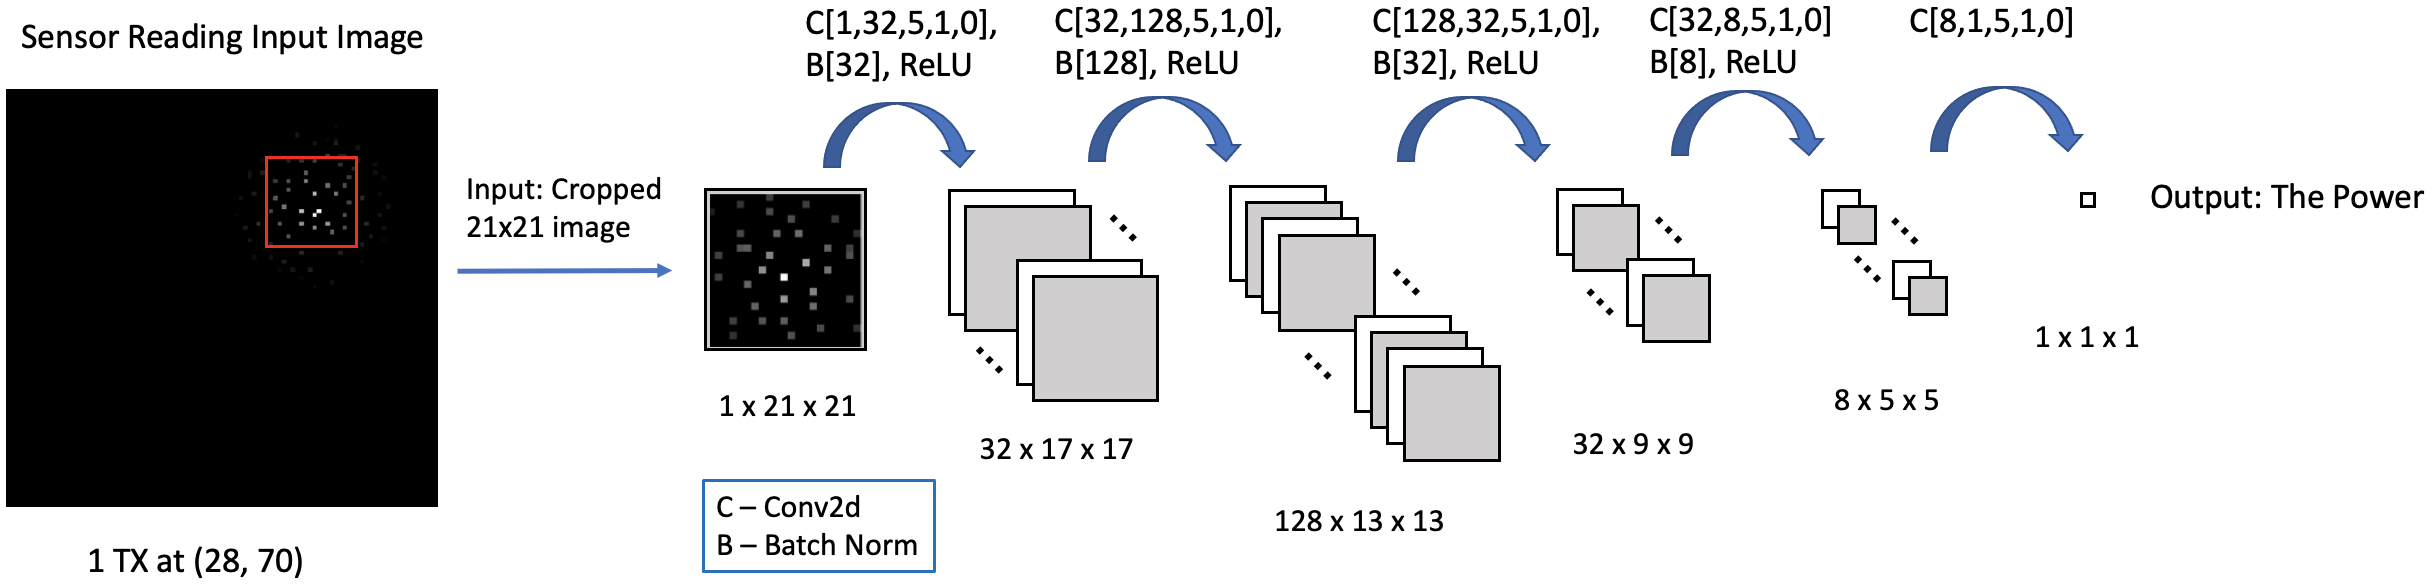
\includegraphics[width=\textwidth]{chapters/wowmom-pmc/figures/power_predictor.png}
    \caption{Architecture of the \power, a five-layer CNN model that takes in a cropped image from the original input image and outputs the predicted power of one transmitter. The figure displays how the data volume flows through the various convolutional layers. C stands for Conv2d, a 2D convolutional layer, and for each Conv2d layer, the five values shown are [number of input channel, number of output channel, kernel size, stride, padding]. B stands for batch normalization 2d, and for each batch normalization, the value shown is [number-of-features].}
    \label{fig:power_predict}
\end{figure}


\softpara{\power CNN Architecture.}
We refer to our CNN model that estimates the power of a single transmitter as \power.
See Fig.~\ref{fig:power_predict}.
It has a similar design to \imgimg as well, where it has no max-pooling layers and no fully connected layers.
We do not use the fully connected layers and design a fully-convolutional network since the usage of fully connected layers will destroy the spatial relationships.
\power has five CNN layers and each CNN layer has a kernel size $5\times5$, striding 1 and padding 0.
With this setting, a pixel in the output layer has a receptive field of $21\times 21$, which is exactly the size of the input cropped image. Also note that the pixel is exactly at the location where the transmitter is assumed to be located (recall that the transmitter is at the center of the cropped image).
We tried both batch normalization and group normalization and found that batch normalization is better than group normalization, which is the opposite to the \imgimg scenario.
ReLU is used as the activation function.
% So each pixel at the output layer can ``see" the entire input image.

{\em Loss Function.} The output of the last convolutional layer is technically a 3D cube, although $1 \times 1 \times 1$. So we flatten it in the end to get one scalar value.
We use a L2 loss function, which is formally defined as:
\begin{equation}
 \frac{1}{N} \sum_{i}^{N} (\power(X^c_{i}) - y_i)^2,
\end{equation}
where $N$ is the number of training samples,~$X^c_{i}$ is the cropped input image for the $i^{th}$ sample and $y_i$ is the ground truth power for the $i^{th}$ sample.
$\power(X^c_{i})$ is the predicted power.
We use Adam as the optimizer, and set the learning rate to 0.001 and the number of epochs to 20, which is sufficient for the model convergence.

\subsection{Estimating Powers of Multiple Transmitters}
Our end goal is to estimate the power of multiple transmitters at the same time. 
When the multiple transmitters are far away and isolated from each other, the problem reduces to single transmitter power estimation, which \power handles well.
The hard part is to estimate transmit powers of multiple transmitters that are close by. 
In this case, a sensor will receive an aggregated power from multiple transmitters. We assume that blind source power separation is not viable. 

\subpara{Overall High-Level Approach}.
For each localized intruder by using \our (whether isolated or not), we crop the $21\times 21$ size area around it and feed it to \power, and estimate its power. If it is actually isolated, then the predicted power is final. If it is not isolated, then we apply a post-processing correction phase to account for the overestimation of the powers, as described below.

\eat{
One idea is to design a CNN model that can directly predicts the power of multiple transmitters.
But this is non-trivial.
Actually, it is the fact that we are having a difficult time directly predicting multiple transmitter power that lead us design \power that only predicts the power a single transmitter.
A core reason is that it requires more complex input and output to predict the power of multiple transmitters, and it is by largely reducing the input and output complexity that we are able to achieve single transmitter power estimation.}

\eat{but To explain the hardness, let's go back to the design choice of \power.
The two key design of \power are that 1) the location of the single transmitter whose power is being estimated is right at the center of the cropped input image and 2) the output of the model is only one pixel whose value is the estimated power of that single transmitter.
However, when a CNN model wishes to directly estimate the power of multiple close by transmitters, two issues arrives:
1) Where to crop the image? You either crop the image centered at one arbitrary transmitter or at the geo-center of multiple close by transmitters.
Or you don't crop at all and take in the whole sensor readings input image, which only increase  the complexity and make the model more difficult to train.
2) The output cannot be a single pixel and must be multiple pixels to represent multiple transmitters.
But the number of close by transmitters is unknown.
So it need multiple models that has a different number of output pixels in the last layer and then do a matching that match a pixel to a specific transmitter.
Image translation based methods introduced in section~\ref{sec:translate} can avoid having multiple models, but it doesn't work well even for the single power estimation.
Given all the difficulties above, we come up with an approach that avoids them and workaround.}

\softpara{Correction Method for Close by Transmitters}.
Let us first consider the case where there are two close by transmitters $T_0$ and $T_1$. We use \power to estimate the power of two transmitters and get $p_0^{'}$ and $p_1^{'}$ respectively.
Let us say the ground truth are $p_0$ and $p_1$ respectively.
The estimated power will most likely be higher than the ground true power, i.e., $p_0^{'} > p_0$ and $p_1^{'} > p_1$.
Because \power can only ``see" one transmitter, and it will view two transmitters in the areas as a combined single one.
Let us focus on $T_0$  and assume $\delta_0 = p_0^{'} - p_0$.
The intuition is that $\delta_0$ has some underlying patterns that we are able to recognize.
We model $\delta_0$ as a function of some features related to $T_0$ and $T_1$.
We model $\delta_0$ as follows,
\begin{equation}
  \delta_0 =   \theta_0 \cdot p_0^{'} + \theta_{(1,1)} \cdot d_{01} + \theta_{(1,2)} \cdot p_1^{'} + \theta_{(1,3)} \cdot \frac{p_1^{'}}{d_{01}} 
  \label{equ:twotxpower}
\end{equation}
where $d_{01}$ is the distance between $T_0$ and $T_1$, and the four $\theta$s are the coefficients for the four terms respectively.
The first term is related to $T_0$ itself, and the other three terms are related to $T_1$.
We observe that the smaller the $d_{01}$, the larger the value of $\delta_0$.
And the bigger the $p_{1}^{'}$, the larger the value of $\delta_0$.
So $d_{01}$ has a negative correlation with $\delta_0$ while $p_{1}^{'}$ has a positive correlation.
$\frac{p_1^{'}}{d_{01}}$ is a combination of two terms to increase the number of features.
We also tried a few other features, but we decided to use only these three features for a close by transmitter as a balance of model accuracy and model complexity.

Equation~\ref{equ:twotxpower} is for the case of one close by transmitter, we then extend the equation to handle multiple close by transmitters in the following Equation~\ref{equ:multitxpower},
\begin{equation}
  \delta_0 =  \theta_0 \cdot p_0^{'} + \sum_{i=1}^{m} ( \theta_{(i,1)} \cdot d_{0i} + \theta_{(i,2)} \cdot p_i^{'} + \theta_{(i,3)} \cdot \frac{p_i^{'}}{d_{0i}})
  \label{equ:multitxpower}
\end{equation}
where $m$ is the number of close by transmitters for $T_0$, the transmitter of interest, $d_{0i}$ is the distance between $T_0$ and close by $T_i$, and $p_i^{'}$ is the uncorrected power predicted by \power. 
For the $i$th close by transmitter, we introduce three terms $ d_{0i},  p_i^{'}, \frac{p_i^{'}}{d_{0i}}$, and assign three coefficients $ \theta_{(i,1)}, \theta_{(i,2)}, \theta_{(i,3)}$ to the three terms respectively.
So for $m$ close by transmitters, there are $1 + 3m$ number of terms in the Equation~\ref{equ:multitxpower}.

After modeling $\delta_0$, in Equation~\ref{equ:correct}, we ``correct'' $p_0^{'}$ by subtracting $\delta_0$ from $p_0^{'}$ to get more an accurate estimation of the power of transmitter $T_0$.
\begin{equation}
    p_{0}^{correct} = p_{0}^{'} - \delta_0
    \label{equ:correct}
\end{equation}

\softpara{Estimating the parameter $\theta$}.
Equation~\ref{equ:multitxpower} is essentially a linear model and we can train it by using either linear, ridge, or LASSO regression models~\cite{scikit-learn}.
We perform experiments using ridge regression (alpha=0.01). 
We set a distance threshold for a neighbor transmitter to be classified as a close by transmitter. 
Note that the transmitters will have a different number of close by transmitters. 
So, let us denote $M$ as the maximum number of close by transmitters we see in the dataset.
When training the linear model in Equation~\ref{equ:multitxpower}, we train a model that assumes a maximum $M$ number of close by transmitters, i.e., the linear model has $1+3M$ terms.
The $3M$ terms are organized in a group of three (i.e., three features) and the groups are sorted by distance in an ascending order.
Then, for a transmitter with a smaller than $M$ number of close by transmitters, let us say $m$, only the first $1+3m$ terms will have a meaningful value.
And for the rest $3(M-m)$ terms, we set the value to zero, i.e., impute missing value with zero.